% Team 02 – Final Presentation: Text Classification & OOD Detection with ModernBERT
% Professional German University Style LaTeX Beamer Presentation

\documentclass[aspectratio=169, 11pt]{beamer}

% ============================================================================
% THEME CONFIGURATION – German University Style
% ============================================================================
\usetheme{Madrid}
\usecolortheme{whale}

% Custom colors inspired by German universities (TU/LMU style)
\definecolor{uniblue}{RGB}{0, 51, 102}
\definecolor{unigray}{RGB}{85, 85, 85}
\definecolor{lightgray}{RGB}{240, 240, 240}
\definecolor{accentred}{RGB}{153, 0, 0}
\definecolor{accentgreen}{RGB}{0, 102, 51}

% Apply custom colors
\setbeamercolor{structure}{fg=uniblue}
\setbeamercolor{frametitle}{bg=uniblue, fg=white}
\setbeamercolor{title}{bg=uniblue, fg=white}
\setbeamercolor{block title}{bg=uniblue, fg=white}
\setbeamercolor{block body}{bg=lightgray, fg=black}
\setbeamercolor{block title alerted}{bg=accentred, fg=white}
\setbeamercolor{block body alerted}{bg=lightgray!50!white, fg=black}
\setbeamercolor{block title example}{bg=accentgreen, fg=white}
\setbeamercolor{block body example}{bg=lightgray!50!white, fg=black}
\setbeamercolor{item}{fg=uniblue}
\setbeamercolor{subitem}{fg=unigray}
\setbeamercolor{footline}{fg=unigray}

% Remove navigation symbols
\setbeamertemplate{navigation symbols}{}

% Custom footline
\setbeamertemplate{footline}{
  \leavevmode%
  \hbox{%
    \begin{beamercolorbox}[wd=.333333\paperwidth,ht=2.25ex,dp=1ex,center]{author in head/foot}%
      \usebeamerfont{author in head/foot}\insertshortauthor
    \end{beamercolorbox}%
    \begin{beamercolorbox}[wd=.333333\paperwidth,ht=2.25ex,dp=1ex,center]{title in head/foot}%
      \usebeamerfont{title in head/foot}\insertshorttitle
    \end{beamercolorbox}%
    \begin{beamercolorbox}[wd=.333333\paperwidth,ht=2.25ex,dp=1ex,right]{date in head/foot}%
      \usebeamerfont{date in head/foot}\insertshortdate{}\hspace*{2em}
      \insertframenumber{} / \inserttotalframenumber\hspace*{2ex}
    \end{beamercolorbox}}%
  \vskip0pt%
}

% ============================================================================
% PACKAGES
% ============================================================================
\usepackage[utf8]{inputenc}
\usepackage[T1]{fontenc}
\usepackage{lmodern}
\usepackage{amsmath, amssymb}
\usepackage{booktabs}
\usepackage{graphicx}
\usepackage{tikz}
\usetikzlibrary{positioning, arrows.meta, calc}
\usepackage{xcolor}
\usepackage{array}
\usepackage{multirow}
\usepackage{hyperref}

% Table column types
\newcolumntype{L}[1]{>{\raggedright\arraybackslash}p{#1}}
\newcolumntype{C}[1]{>{\centering\arraybackslash}p{#1}}
\newcolumntype{R}[1]{>{\raggedleft\arraybackslash}p{#1}}

% ============================================================================
% TITLE PAGE INFORMATION
% ============================================================================
\title[BERT Text Classification]{Multi-Class Text Classification with BERT}
\author[Team]{ M. Nasim Palakka Valappil \& Ganesh Yadav Yatham }
\institute[Universit\"at Bremen]{ Advanced Machine Learning\\Winter Semester 2025/26}
\date{March 3, 2026}

% ============================================================================
% DOCUMENT
% ============================================================================
\begin{document}

% ------ Title Slide ------
\begin{frame}[plain]
  \titlepage
\end{frame}

% ------ Outline ------
\begin{frame}{Outline}
  \tableofcontents
\end{frame}

% ============================================================================
\section{Problem Statement}
% ============================================================================

\begin{frame}{Problem Statement}

  \textbf{\large Task}

  \vspace{0.3cm}

  \begin{itemize}
    \item \textbf{Multi-class text classification} on the 20 Newsgroups dataset \\ (20~newsgroup categories)
    \item \textbf{Open-world extension:} detect inputs that do \emph{not} belong to any of the 20 known categories
  \end{itemize}

  \vspace{0.6cm}

  \textbf{\large Approach}

  \vspace{0.3cm}

  \begin{enumerate}
    \item Fine-tune a \textbf{pre-trained foundational transformer model} (ModernBERT)
    \item Systematically optimise hyperparameters with \textbf{Quasi-Random Search}
    \item Extend to OOD detection using \textbf{Maximum Softmax Probability (MSP)}
  \end{enumerate}
\end{frame}

% ============================================================================
\section{Dataset Overview}
% ============================================================================

\begin{frame}{Dataset: 20 Newsgroups -- Overview}
  \begin{columns}[T]
    \begin{column}{0.42\textwidth}
      \footnotesize
      \renewcommand{\arraystretch}{1.15}
      \begin{tabular}{@{}l l@{}}
        \toprule
        \textbf{Property} & \textbf{Value} \\
        \midrule
        Source        & \texttt{SetFit/20\_newsgroups} \\
        Classes       & 20 newsgroup categories \\
        Train samples & 11\,314 \\
        Test samples  & 7\,532 \\
        Total         & 18\,846 \\
        \bottomrule
      \end{tabular}
    \end{column}

    \begin{column}{0.55\textwidth}
      \textbf{Category groups}
      \footnotesize
      \begin{itemize}
        \item \textbf{Computer (5):} \texttt{comp.graphics}, \texttt{comp.os.ms-windows.misc}, \texttt{comp.sys.ibm.pc.hardware}, \texttt{comp.sys.mac.hardware}, \texttt{comp.windows.x}
        \item \textbf{Recreation (4):} \texttt{rec.autos}, \texttt{rec.motorcycles}, \texttt{rec.sport.baseball}, \texttt{rec.sport.hockey}
        \item \textbf{Science (4):} \texttt{sci.crypt}, \texttt{sci.electronics}, \texttt{sci.med}, \texttt{sci.space}
        \item \textbf{Politics / Religion (6):} \texttt{talk.politics.*}, \texttt{alt.atheism}, \texttt{soc.religion.christian}
        \item \textbf{Other (1):} \texttt{misc.forsale}
      \end{itemize}
    \end{column}
  \end{columns}
\end{frame}

\begin{frame}{Dataset -- Splits and Statistics}
  \begin{columns}[T]
    \begin{column}{0.48\textwidth}
      \footnotesize
      \renewcommand{\arraystretch}{1.15}
      \begin{tabular}{@{}l c l@{}}
        \toprule
        \textbf{Split} & \textbf{Size} & \textbf{Purpose} \\
        \midrule
        Train      & 11\,314 & Model training \\
        Validation & 3\,766  & HPO \& model selection \\
        Test       & 3\,766  & Final held-out evaluation \\
        \bottomrule
      \end{tabular}

      \vspace{0.4cm}

      \renewcommand{\arraystretch}{1.15}
      \begin{tabular}{@{}l c c@{}}
        \toprule
        \textbf{Metric} & \textbf{Characters} & \textbf{Words} \\
        \midrule
        Mean   & $\sim$1\,800 & $\sim$300 \\
        Median & $\sim$900    & $\sim$150 \\
        P95    & $\sim$6\,500 & $\sim$1\,100 \\
        \bottomrule
      \end{tabular}
    \end{column}

    \begin{column}{0.48\textwidth}
      \textbf{Tokenisation coverage} (\texttt{max\_length})

      \vspace{0.2cm}

      \begin{itemize}
        \item 128 tokens $\rightarrow$ $\sim$50\,\% coverage
        \item \textbf{256 tokens $\rightarrow$ $\sim$75\,\% coverage} $\;\leftarrow$ chosen
        \item 512 tokens $\rightarrow$ $\sim$90\,\% coverage
      \end{itemize}

      \vspace{0.3cm}

      \footnotesize
      \begin{itemize}
        \item[\textcolor{accentgreen}{+}] Manageable training time and computational cost
        \item[\textcolor{accentgreen}{+}] First 256 tokens are generally sufficient to predict the label
        \item[\textcolor{accentred}{--}] Some information loss for very long documents
      \end{itemize}
    \end{column}
  \end{columns}
\end{frame}

% ============================================================================
\section{Model: ModernBERT}
% ============================================================================

\begin{frame}{Model: ModernBERT}
  Recent \textbf{encoder-only} model by HuggingFace -- a modernised version of BERT with multiple architectural improvements for robustness and efficiency.

  \vspace{0.4cm}

  \begin{columns}[T]
    \begin{column}{0.42\textwidth}
      \textbf{BERT $\rightarrow$ RoBERTa}

      \vspace{0.15cm}

      \begin{itemize}
        \item Significantly more training data
        \item No Next Sentence Prediction loss
        \item Dynamic masking
      \end{itemize}
    \end{column}

    \begin{column}{0.54\textwidth}
      \textbf{RoBERTa $\rightarrow$ ModernBERT}

      \vspace{0.15cm}

      \begin{itemize}
        \item Even more training data
        \item \textbf{GeGLU} activation (more robust than GeLU)
        \item No bias terms except in last linear layer
        \item \textbf{Pre-normalisation} (LayerNorm at the beginning of sub-layers)
        \item Alternating attention
      \end{itemize}
    \end{column}
  \end{columns}
\end{frame}

% ============================================================================
\section{Training Strategy}
% ============================================================================

\begin{frame}{Training Strategy}
  \begin{columns}[T]
    \begin{column}{0.44\textwidth}
      \textbf{Layer Freezing}

      \vspace{0.2cm}

      \footnotesize
      \renewcommand{\arraystretch}{1.15}
      \begin{tabular}{@{}l l@{}}
        \toprule
        \textbf{Component} & \textbf{Status} \\
        \midrule
        Embedding layer      & Frozen \\
        Encoder layers 0--13 & Frozen (bottom 50\%) \\
        Encoder layers 14--27 & Trainable (top 50\%) \\
        Classification head  & Trainable \\
        \bottomrule
      \end{tabular}

      \vspace{0.3cm}
      \scriptsize
      Further unfreezing layers significantly increased compute requirements without meaningful accuracy gains.
    \end{column}

    \begin{column}{0.52\textwidth}
      \textbf{Training Configuration}

      \vspace{0.2cm}

      \footnotesize
      \renewcommand{\arraystretch}{1.15}
      \begin{tabular}{@{}l l@{}}
        \toprule
        \textbf{Parameter} & \textbf{Value} \\
        \midrule
        Optimiser        & AdamW \\
        Epochs           & 4 \\
        Batch size       & 16 per GPU \\
        Max sequence len  & 256 tokens \\
        Mixed precision  & FP16 (CUDA) \\
        Gradient clipping & max\_norm = 1.0 \\
        LR scheduler     & Linear warmup + decay \\
        Hardware         & NVIDIA Tesla T4 \\
        Multi-GPU        & \texttt{nn.DataParallel} \\
        \bottomrule
      \end{tabular}
    \end{column}
  \end{columns}
\end{frame}

% ============================================================================
\section{Hyperparameter Optimisation}
% ============================================================================

\begin{frame}{Hyperparameter Optimisation}
  \begin{columns}[T]
    \begin{column}{0.48\textwidth}
      \textbf{Method~1:} Hyperparameters from the original ModernBERT paper, theory, and intuition.

      \vspace{0.4cm}

      \textbf{Method~2: Quasi-Random Search (QRS) via Optuna}

      \vspace{0.15cm}

      \begin{itemize}
        \item Better space coverage than grid or pure random search
        \item Uses \textbf{Quasi-Monte Carlo (QMC)} sampling for low-discrepancy sequences
        \item More efficient exploration of the hyperparameter landscape
      \end{itemize}
    \end{column}

    \begin{column}{0.48\textwidth}
      \textbf{Search Space}

      \vspace{0.2cm}

      \footnotesize
      \renewcommand{\arraystretch}{1.15}
      \begin{tabular}{@{}l l l@{}}
        \toprule
        \textbf{Hyperparameter} & \textbf{Range} & \textbf{Scale} \\
        \midrule
        Learning rate & $[10^{-5},\, 10^{-4}]$ & Log \\
        Weight decay  & $[0.001,\, 0.1]$        & Linear \\
        Warmup ratio  & $[0.0,\, 0.2]$          & Linear \\
        \bottomrule
      \end{tabular}

      \vspace{0.4cm}

      \normalsize
      \textbf{Setup}
      \begin{itemize}
        \item Objective: \textbf{maximise validation accuracy}
        \item Aggressive memory management (delete non-top-3 checkpoints)
        \item Optuna visualisations: slice plots \& parameter importance
      \end{itemize}
    \end{column}
  \end{columns}
\end{frame}

\begin{frame}{HPO -- Visualisation and Evaluation}
  \begin{columns}[T]
    \begin{column}{0.48\textwidth}
      \centering
      \textbf{Hyperparameters vs. Loss}

      \vspace{0.15cm}

      \includegraphics[width=0.95\textwidth]{qrs_hyperparameters_vs_loss.png}

      \vspace{0.4cm}

      \textbf{Test-Set Performance}

      \vspace{0.15cm}

      \scriptsize
      \renewcommand{\arraystretch}{1.15}
      \begin{tabular}{@{}l c c c@{}}
        \toprule
        \textbf{Metric} & \textbf{Top-1} & \textbf{Top-2} & \textbf{Top-3} \\
        \midrule
        Accuracy    & 74.93\% & 74.35\% & 73.26\% \\
        Macro F1    & 0.7385  & 0.7353  & 0.7246  \\
        Weighted F1 & 0.7486  & 0.7453  & 0.7344  \\
        Test Loss   & 1.2554  & 1.4491  & 1.6971  \\
        \bottomrule
      \end{tabular}
    \end{column}

    \begin{column}{0.48\textwidth}
      \centering
      \textbf{Parameter Importances}

      \vspace{0.2cm}

      \includegraphics[width=\textwidth]{qrs_param_importances.png}
    \end{column}
  \end{columns}
\end{frame}

% ============================================================================
\section{Evaluation on Additional Modern Forum Data}
% ============================================================================

\begin{frame}{Evaluation on Additional Modern Forum Data}
\begin{itemize}
\item Collected a few samples for each class using web scrapers and a few samples manually from subReddits.
\item Total of \textbf{2,000 samples} were collected (100 samples for each class) and stored in \texttt{collected\_reddit\_data.csv}.
\item Evaluated the Top-2 model on \texttt{collected\_reddit\_data.csv}.
\end{itemize}

\vspace{0.3cm}

\textbf{Evaluation Results:}
\begin{itemize}
\item Test Loss: \textbf{0.9896}
\item Accuracy: \textbf{0.7800}
\end{itemize}

\vspace{0.2cm}

\begin{center}
\renewcommand{\arraystretch}{1.2}
\begin{tabular}{@{}l c c c@{}}
\toprule
\textbf{Metric} & \textbf{Test Set} & \textbf{Reddit} & \textbf{Change} \\
\midrule
Accuracy    & 0.7435 & 0.7800 & +0.0365 \\
Macro F1    & 0.7353 & 0.7700 & +0.0347 \\
Weighted F1 & 0.7453 & 0.7700 & +0.0248 \\
\bottomrule
\end{tabular}
\end{center}
\end{frame}

% ============================================================================
\section{Key Findings}
% ============================================================================

\begin{frame}{Key Findings \& Interpretation}
  \textbf{Test Set vs. Collected Reddit Data}

  \vspace{0.2cm}

  \begin{columns}[T]
    \begin{column}{0.48\textwidth}
      \textbf{1. Categories with Large Improvements}
      \begin{itemize}
        \footnotesize
        \item \texttt{rec.autos} (+0.293)
        \item \texttt{talk.politics.misc} (+0.315)
        \item \texttt{talk.politics.guns} (+0.244)
        \item \texttt{sci.electronics} (+0.219)
        \item \texttt{rec.motorcycles} (+0.148)
        \item \texttt{sci.space} (+0.152)
        \item \texttt{rec.sport.baseball} (+0.115)
        \item \texttt{sci.crypt} (+0.100)
      \end{itemize}

      \vspace{0.2cm}
      \textbf{2. Categories with Moderate Gains}
      \begin{itemize}
        \footnotesize
        \item \texttt{alt.atheism} (+0.060)
        \item \texttt{comp.graphics} (+0.049)
        \item \texttt{comp.sys.mac.hardware} (+0.016)
        \item \texttt{rec.sport.hockey} (+0.050)
        \item \texttt{talk.politics.mideast} (+0.034)
        \item \texttt{sci.med} (+0.086)
      \end{itemize}
    \end{column}

    \begin{column}{0.48\textwidth}
      \textbf{3. Categories with Declines}
      \begin{itemize}
        \footnotesize
        \item \texttt{comp.windows.x} (--0.328)
        \item \texttt{comp.sys.ibm.pc.hardware} (--0.259)
        \item \texttt{misc.forsale} (--0.230)
        \item \texttt{soc.religion.christian} (--0.163)
        \item \texttt{talk.religion.misc} (--0.131)
        \item \texttt{comp.os.ms-windows.misc} (--0.077)
      \end{itemize}

      \vspace{0.2cm}
      \textbf{4. Factors Influencing Performance}
      \begin{itemize}
        \footnotesize
        \item Subreddit relevance
        \item Temporal language shift
        \item Community norms
        \item Class imbalance in original data
      \end{itemize}
    \end{column}
  \end{columns}
\end{frame}

% ============================================================================
\section{Confidence Analysis}
% ============================================================================

\begin{frame}{Confidence Score \& Certainty of the Model}
  \textbf{Maximum Softmax Probability (MSP)}

  \vspace{0.2cm}

  Confidence computed using Softmax:
  \[
  P(y=i) = \frac{e^{z_i}}{\sum_{j} e^{z_j}}
  \]

  \textbf{Confidence score} = Maximum Softmax Probability (MSP)

  \vspace{0.2cm}
  Evaluated on full test set.

  \vspace{0.4cm}

  \textbf{Results:}
  \begin{itemize}
    \item \textbf{Avg Confidence (Correct):} 0.9508
    \item \textbf{Avg Confidence (Incorrect):} 0.6879
    \item \textbf{Correlation (Confidence vs Correctness):} 0.5384
  \end{itemize}

  \vspace{0.2cm}
  \begin{center}
    \textit{The model is significantly less confident when it makes a mistake.}
  \end{center}
\end{frame}

% ============================================================================

\begin{frame}{Confidence Score \& Certainty of the Model}
  \textbf{Test-Time Augmentation (TTA) for Uncertainty Estimation}

  \begin{enumerate}
    \item Apply 10 stochastic augmentations to each test sample
    \item Run model inference on each augmented version
    \item Average predicted probability distributions
    \item Compute predictive entropy from the averaged probabilities
    \item Compare entropy for correct vs incorrect predictions
  \end{enumerate}

  \vspace{0.2cm}

  \textbf{Predictive Entropy Formula}
  \[
  H(p) = -\sum_{i=1}^{C} p_i \log p_i
  \]
  Where $p_i$ = averaged predicted probability for class $i$, and $C$ = number of classes. \\
  \textit{Higher $H(p)$ $\rightarrow$ higher uncertainty.}

  \vspace{0.3cm}

  \textbf{Results:}
  \begin{itemize}
    \item \textbf{Avg entropy (Correct):} 0.1424
    \item \textbf{Avg entropy (Incorrect):} 0.9232
    \item \textbf{Difference:} 0.7808
  \end{itemize}
\end{frame}

% ============================================================================
\section{Out-of-Distribution Detection}
% ============================================================================

\begin{frame}{Out-of-Distribution Detection}
  \textbf{Strategy: Maximum Softmax Probability (MSP)}

  \vspace{0.2cm}

  $$\text{score}(x) = \max_k \; \text{softmax}\!\left(\frac{\mathbf{z}(x)}{T}\right)_k$$

  \begin{itemize}
    \item \textbf{If} $\text{score}(x) \geq \tau$ $\;\rightarrow\;$ classify as one of the 20 classes \textcolor{accentgreen}{(In-Distribution)}
    \item \textbf{If} $\text{score}(x) < \tau$ $\;\rightarrow\;$ reject as \textbf{``null / other''} \textcolor{accentred}{(Out-of-Distribution)}
  \end{itemize}

  \vspace{0.3cm}

  \footnotesize
  \renewcommand{\arraystretch}{1.15}
  \begin{tabular}{@{}l L{11cm}@{}}
    \toprule
    \textbf{Parameter} & \textbf{Effect} \\
    \midrule
    Temperature $T$ & $T > 1$: softens probabilities $\rightarrow$ better ID/OOD separation \\
    Threshold $\tau$ & Higher $\tau$: stricter $\rightarrow$ fewer false positives, more false negatives \\
    \bottomrule
  \end{tabular}
\end{frame}

\begin{frame}{OOD Detection Setup}
  \begin{columns}[T]
    \begin{column}{0.48\textwidth}
      \textbf{In-Distribution (ID)}
      \begin{itemize}
        \item \textbf{20~Newsgroups test set} (3\,766 samples)
        \item Same split used for classification evaluation
      \end{itemize}

      \vspace{0.4cm}

      \textbf{Out-of-Distribution (OOD)}
      \begin{itemize}
        \item \textbf{AG News} -- 4-class news topic classification
        \item 2\,000 randomly sampled test documents
        \item \textbf{Completely different domain} from 20~Newsgroups
      \end{itemize}
    \end{column}

    \begin{column}{0.48\textwidth}
      \textbf{Evaluation Protocol}

      \vspace{0.15cm}

      \begin{enumerate}
        \item Collect model logits for both ID and OOD data
        \item Compute MSP scores at temperatures $T \in \{6, 7, 8, 9, 10\}$
        \item For each $T$, report:
          \begin{itemize}
            \item \textbf{AUROC} (Area Under ROC Curve)
            \item \textbf{AP} (Average Precision)
            \item \textbf{FPR@TPR70}
          \end{itemize}
        \item Per-threshold table: FPR, FNR, retained ID accuracy, \% ID kept
      \end{enumerate}
    \end{column}
  \end{columns}
\end{frame}

\begin{frame}{OOD Detection -- The FP\,/\,FN Trade-off}
  \begin{columns}[T]
    \begin{column}{0.44\textwidth}
      \textbf{Understanding the Threshold $\tau$}

      \vspace{0.2cm}

      \footnotesize
      \renewcommand{\arraystretch}{1.15}
      \begin{tabular}{@{}l l l@{}}
        \toprule
        \textbf{Direction} & \textbf{Effect} & \textbf{Consequence} \\
        \midrule
        $\uparrow\;\tau$ & Stricter & \textcolor{accentgreen}{$\downarrow$ FP}\;/\;\textcolor{accentred}{$\uparrow$ FN} \\
        $\downarrow\;\tau$ & Looser  & \textcolor{accentgreen}{$\downarrow$ FN}\;/\;\textcolor{accentred}{$\uparrow$ FP} \\
        \bottomrule
      \end{tabular}

      \vspace{0.4cm}
      \normalsize
      \centering
      \textit{The optimal operating point depends on tolerance for false positives vs.\ false negatives.}
    \end{column}

    \begin{column}{0.52\textwidth}
      \textbf{Threshold Table} ($T = 6.00$)

      \vspace{0.1cm}

      \tiny
      AUROC\,=\,0.7961 \quad AP\,=\,0.8841 \quad FPR@TPR70\,=\,0.2050

      \vspace{0.15cm}

      \footnotesize
      \renewcommand{\arraystretch}{1.1}
      \begin{tabular}{@{}c c c c c@{}}
        \toprule
        $\tau$ & FPR & FNR & ID Acc & \% ID \\
        \midrule
        0.10 & 0.875 & 0.052 & 0.785 & 94.8\% \\
        0.20 & 0.263 & 0.249 & 0.874 & 75.1\% \\
        0.30 & 0.105 & 0.481 & 0.942 & 51.9\% \\
        0.40 & 0.031 & 0.720 & 0.974 & 28.0\% \\
        0.50 & 0.000 & 0.943 & 0.991 & 5.7\% \\
        \bottomrule
      \end{tabular}
    \end{column}
  \end{columns}
\end{frame}

\begin{frame}{OOD Detection -- Diagnostic Visualisations}
  \textbf{Three diagnostic plots} are generated per temperature:

  \vspace{0.1cm}

  \begin{center}
    \includegraphics[width=\textwidth]{ood_detection_T0600.png}
  \end{center}

  \vspace{0.1cm}

  \begin{columns}[T]
    \begin{column}{0.30\textwidth}
      \centering
      \textbf{1.\;ROC Curve}

      \vspace{0.2cm}

      \footnotesize
      \begin{itemize}
        \item AUROC summarises discriminative quality
        \item Annotated with FPR@TPR70
      \end{itemize}
    \end{column}

    \begin{column}{0.36\textwidth}
      \centering
      \textbf{2.\;Confidence Distributions}

      \vspace{0.2cm}

      \footnotesize
      \begin{itemize}
        \item Good detection $\rightarrow$ well-separated distributions
        \item OOD should cluster at lower confidence
      \end{itemize}
    \end{column}

    \begin{column}{0.30\textwidth}
      \centering
      \textbf{3.\;FP\,/\,FN Trade-off}

      \vspace{0.2cm}

      \footnotesize
      \begin{itemize}
        \item Crossing point = balanced operating point
        \item Select $\tau$ per application needs
      \end{itemize}
    \end{column}
  \end{columns}
\end{frame}

% ============================================================================

% ============================================================================

\begin{frame}{Results -- OOD Temperature Comparison}
  \begin{center}
    \renewcommand{\arraystretch}{1.2}
    \begin{tabular}{@{}c c c c@{}}
      \toprule
      \textbf{Temperature $T$} & \textbf{AUROC} & \textbf{AP} & \textbf{FPR@TPR70} \\
      \midrule
      6.00  & 0.7961 & 0.8841 & 0.2050 \\
      7.00  & 0.7986 & 0.8860 & 0.2000 \\
      8.00  & 0.8003 & 0.8875 & 0.1970 \\
      9.00  & 0.8016 & 0.8885 & 0.1930 \\
      \textbf{10.00} & \textbf{0.8026} & \textbf{0.8893} & \textbf{0.1910} \\
      \bottomrule
    \end{tabular}

    \vspace{0.5cm}

    Higher temperatures yield modest improvements across all metrics.\\[0.15cm]
    Best performance at $T = 10$:\; AUROC\,=\,0.8026,\; AP\,=\,0.8893,\; FPR@TPR70\,=\,0.1910
  \end{center}
\end{frame}

% ============================================================================
\section{Key Design Decisions}
% ============================================================================

\begin{frame}{Key Design Decisions}
  \begin{enumerate}
    \item \textbf{Used ModernBERT Variant of BERT}
    \begin{itemize}
      \item Version of BERT that includes multiple small tweaks to make the transformer architecture more robust and efficient
    \end{itemize}

    \vspace{0.15cm}

    \item \textbf{Layer Freezing (50\%)}
    \begin{itemize}
      \item Faster training, less memory $\rightarrow$ allows larger batch size
      \item Minimal accuracy loss: lower layers learn general language features
    \end{itemize}

    \vspace{0.15cm}

    \item \textbf{Initial Hyperparameters from ModernBERT Architecture}
    \begin{itemize}
      \item Seeded tuning process with parameters proven effective in original paper
    \end{itemize}

    \vspace{0.15cm}

    \item \textbf{Quasi-Random Search (QRS) over Grid/Random}
    \begin{itemize}
      \item QMC sampling provides \textbf{better coverage} of the search space
    \end{itemize}

    \vspace{0.15cm}

    \item \textbf{Validation Split from Test Set}
    \begin{itemize}
      \item Split test 50/50 $\rightarrow$ separates validation for HPO and final test eval
      \item Prevents data leakage: HPO decisions never touch the test set
    \end{itemize}
  \end{enumerate}
\end{frame}

% ============================================================================
\section{Pipeline Summary}
% ============================================================================

\begin{frame}{Pipeline Summary}
  \begin{center}
    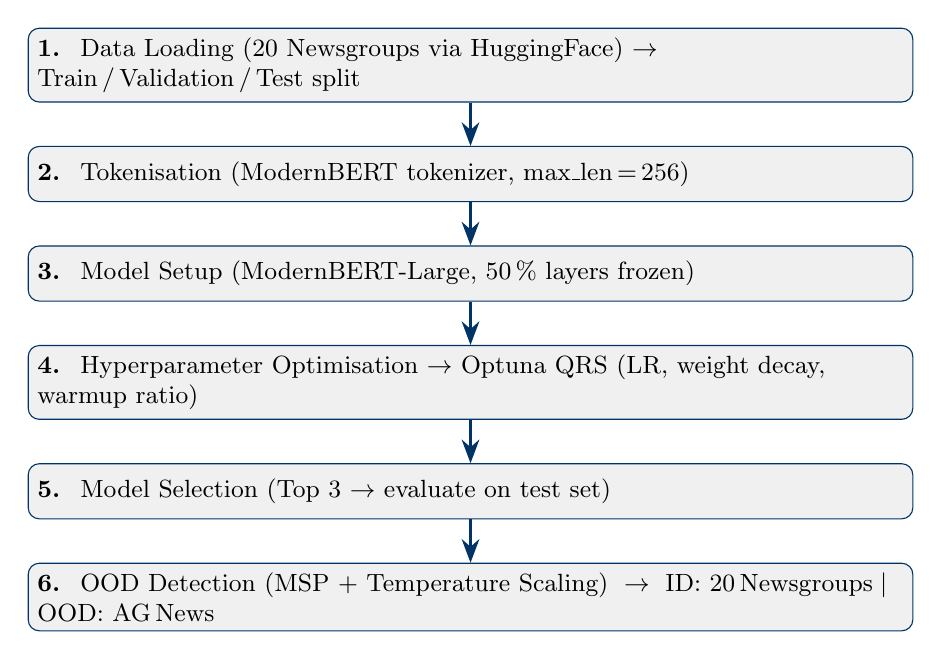
\begin{tikzpicture}[
      node distance=0.55cm,
      box/.style={
        draw=uniblue, fill=lightgray, rounded corners,
        text width=11cm, minimum height=0.7cm,
        align=left, font=\small
      }
    ]
      \node[box] (s1) {\textbf{1.}\; Data Loading (20 Newsgroups via HuggingFace) $\rightarrow$ Train\,/\,Validation\,/\,Test split};
      \node[box, below=of s1] (s2) {\textbf{2.}\; Tokenisation (ModernBERT tokenizer, max\_len\,=\,256)};
      \node[box, below=of s2] (s3) {\textbf{3.}\; Model Setup (ModernBERT-Large, 50\,\% layers frozen)};
      \node[box, below=of s3] (s4) {\textbf{4.}\; Hyperparameter Optimisation $\rightarrow$ Optuna QRS (LR, weight decay, warmup ratio)};
      \node[box, below=of s4] (s5) {\textbf{5.}\; Model Selection (Top~3 $\rightarrow$ evaluate on test set)};
      \node[box, below=of s5] (s6) {\textbf{6.}\; OOD Detection (MSP + Temperature Scaling)\; $\rightarrow$\; ID: 20\,Newsgroups\;\textbar\; OOD: AG\,News};

      \draw[-{Stealth[length=3mm]}, thick, uniblue] (s1) -- (s2);
      \draw[-{Stealth[length=3mm]}, thick, uniblue] (s2) -- (s3);
      \draw[-{Stealth[length=3mm]}, thick, uniblue] (s3) -- (s4);
      \draw[-{Stealth[length=3mm]}, thick, uniblue] (s4) -- (s5);
      \draw[-{Stealth[length=3mm]}, thick, uniblue] (s5) -- (s6);
    \end{tikzpicture}
  \end{center}
\end{frame}



% ============================================================================
\section{Conclusion}
% ============================================================================

\begin{frame}{Conclusion}
  \textbf{Summary}

  \vspace{0.2cm}

  \begin{itemize}
    \item Successfully fine-tuned \textbf{ModernBERT-Large} on 20~Newsgroups (20-class classification)
    \item Systematic \textbf{hyperparameter optimisation} with Optuna Quasi-Random Search
    \item Extended to \textbf{OOD detection} using MSP with temperature scaling
    \item Comprehensive evaluation with AUROC, AP, FPR@TPR70, and threshold analysis
  \end{itemize}

  \vspace{0.5cm}

  \begin{columns}[T]
    \begin{column}{0.48\textwidth}
      \textbf{Future Work}

      \vspace{0.2cm}

      \begin{itemize}
        \item More trials of quasi-random search
        \item Bayesian HPO
        \item Experiment with other BERT variants
      \end{itemize}
    \end{column}

    \begin{column}{0.48\textwidth}
      \begin{alertblock}{Lesson Learned}
        Errors in training pipeline can be very costly when running Optuna Quasi-Random HPO on large transformer models, as each iteration can take hours to run.
      \end{alertblock}
    \end{column}
  \end{columns}
\end{frame}

% ============================================================================

\begin{frame}[plain]
  \begin{center}
    \vfill
    {\Large\textcolor{uniblue}{\textbf{Thank You!}}}

    \vspace{0.6cm}

    {\large Team -- M. Nasim Palakka Valappil \& Ganesh Yadav Yatham }

    \vspace{0.4cm}

    {\normalsize Questions?}
    \vfill
  \end{center}
\end{frame}

\end{document}